\nfch{Ongoing research:}{\~Optimal-Time Incremental}{\Huge Voronoi Diagrams}

\begin{frame} \frametitle{Divide-and-conquer} \vspace{1.2mm}
Time complexity $\Ot(N^{\frac34})$ is not bad, but the lower bound is $N^{\frac12}$. Can we meet it? \\ \smallskip
The idea is to use divide-and-conquer approach. It can allow us to omit \\
doing unnecessary work. \bigskip

\begin{tabular}{lll}
\makecell[c]{
	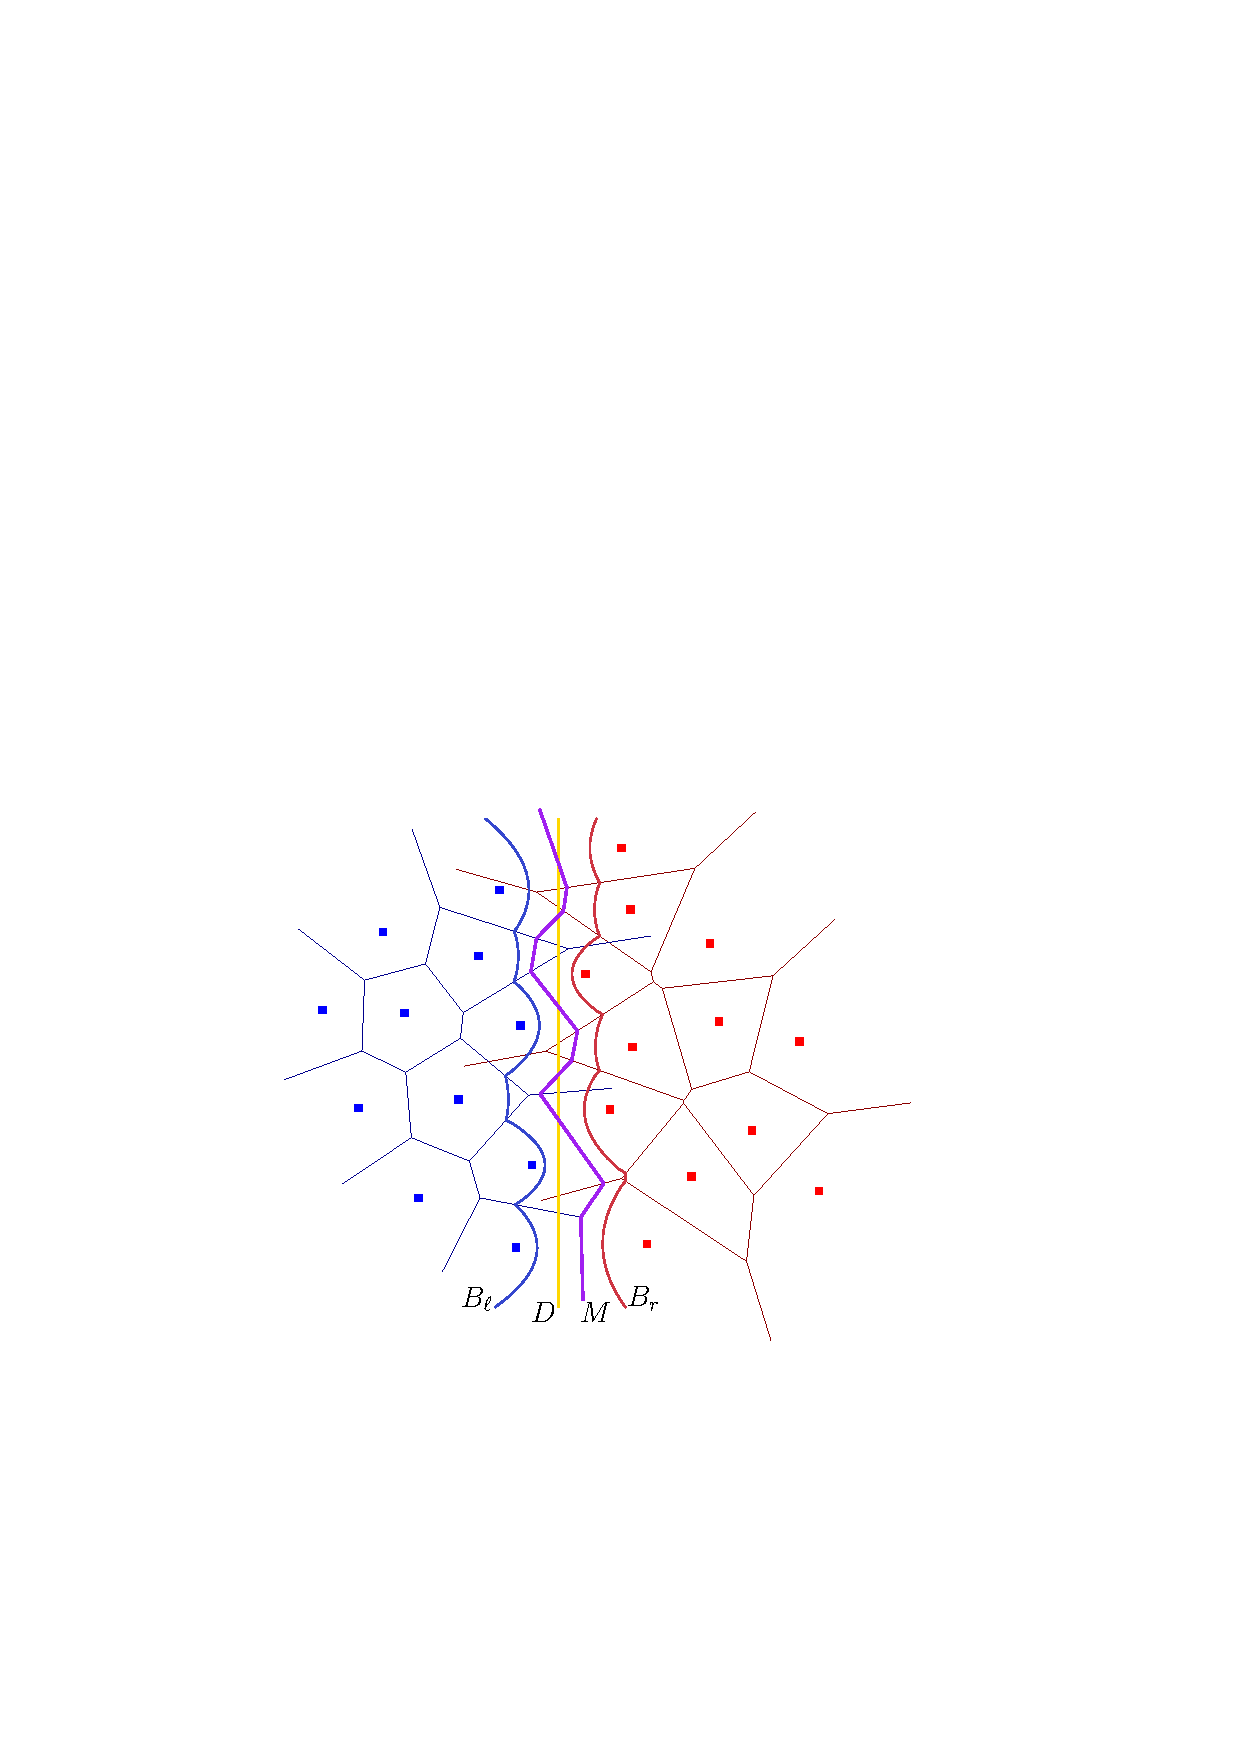
\includegraphics[width=7.5cm]{figs/example}
} & \hspace{0.8cm} & \pause
\makecell[l]{
	\fitem{1}{Dividing line,}
	\fitem{2}{Beach lines,}
	\fitem{3}{Blue and red forests,}
	\fitem{4}{Merge curve.} \phantom{x} \\
}
\end{tabular}
\end{frame}